\section{Voruntersuchung}

\subsection{IST-Erhebung}

Es wird bereits ein Gro�teil des Kapitals in Wertpapieren algorithmisch verwaltet. Daher existiert eine Unmenge an Wissen �ber den Aufbau
von B�rsenalgorithmen und die Anwendung von Indikatoren zur Einsch�tzung von zuk�nftigen Kurswerten. Die meisten dieser Algorithmen basieren auf technischer
Analyse und den simplen Algorithmen die diese mit sich bringt.Bekannte Vertreter davon sind zum Beispiel der MACD und der CCI.
Die meisten Algorithmen benutzen au�erdem eine Zusammensetzung aus verschiedenen \glspl{ma}, um die zu Grunde liegenden Handelsentscheidungen zu treffen.
Aufgrund dieses umfangreichen Wissens ist es m�glich weitere M�glichkeiten zu erforschen und noch besser und sinnvoller handelnde maschinelle Helfer zu kreieren.\\
\\
Ein Problem der aktuellen Situation ist allerdings, das schlechte bzw. umst�ndliche Testing dieser Algorithmen, da wenig Software existiert, die
verifizieren kann ob ein Algorithmus in bestimmten Marktphasen bestimmte Leistungen erbringt. Au�erdem ist es momentan ziemlich kompliziert sich einfach
die gesamte Performance eines solchen Handelsalgorithmus anzusehen. Es gibt hierf�r aber sowohl Gratisquellen, als auch kommerzielle Produkte, von denen man
historische Daten zum Backtesting dar Algorithmen beziehen kann. Das Projektteam von Noctua besitzt bereits ca. 3.9 Gb an historischen B�rsenkursen von
e-Signal \footnote{http://www.esignal.com/default.aspx?tc=} und nahezu unbegrenzten Zugriff auf weitere Daten vom selben Anbieter.
Dadurch ist es ihm m�glich Algorithmen �ber ein weites Spektrum von Marktphasen und -zust�nden hinweg zu testen und die Performance verschiedener Algorithmen in unterschiedlichen Situationen akkurat festzustellen. Dies ist besonders wichtig, da Algorithmen die in der nahen Vergangenheit guten Entscheidungen trafen, meist weiterhin sehr erfolgreich handeln und den Anleger m�glicherweise mit einem Kapitalzuwachs belohnen.

\subsection{IST-Zustand}

Aufgrund der riesingen Industrie die diesem Projekt zu Grunde liegt gibt es nat�rlich bereits eine Vielzahl an Konkurrenzprodukten auf dem Markt. Einige davon spezialisieren sich auf das Backtesting bzw. die Bereitstellung einer Plattform zur Entwicklung von Algorithmen. Andere sind eher propriet�rer Natur und versuchen lediglich durch Korruption der Konkurrenz, selbst den wirtschaftlich rentabelsten Algorithmus zu betreiben. Doch alle haben ihre Vor- und Nachteile. Daher finden sich auch immer wieder neue Nieschen f�r Neueinsteiger am Markt, die durch ausgekl�gekte Algorithmen viel erreichen k�nnen. Im folgenden werden nun die bekanntesten dieser Konkurrenzprodukte berschrieben.

\subsubsection{MetaTrader 5}

Hierbei handelt es sich um ein ziemlich umfangreiches, ein wenig �lteres Produkt, dass sowohl Aktien- als auch Forex-Daten anbietet. MetaTrader 5 ist die neue verbesserte Version von Metatrader 4 und bietet neben den alten Funktionen, Neuerungen wie die Einbindung von News. Au�erdem bietet der MetaTrader ein weites Spektrum an Indikatoren, die einfach in den laufenden Betrieb eingebunden werden k�nnen. Die Oberfl�che des MetaTraders sieht in etwa aus, wie in Abbildung \ref{fig:metatrader5_overview} dargestellt.

\begin{figure}
	\centering
		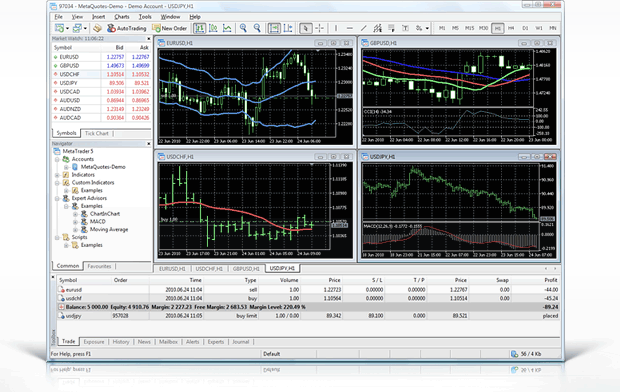
\includegraphics{graphics/chapter2/metatrader5_overview.png}
	\caption{MetaTrader 5 Oberfl�che}
	\label{fig:metatrader5_overview}
\end{figure}

\begin{figure}
	\centering
		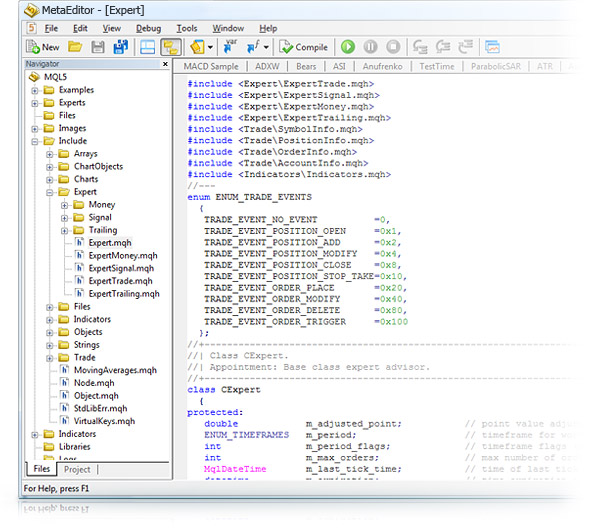
\includegraphics{graphics/chapter2/metaeditor_robot_modification.jpg}
	\caption{MetaTrader 5 IDE-Oberfl�che}
	\label{fig:metaeditor_robot_modification.jpg}
\end{figure}

Doch das gr��te Feature des MetaTraders ist die eingebaute IDE(siehe Abbildung \ref{fig:metaeditor_robot_modification.jpg}), die es mittels einer eigenen MetaTrader-spezifischen Sprache, der \gls{mql5}, erm�glicht eigene Algorithmen zu programmieren und diese dann auch direkt in den laufenden Betrieb zu �bernehmen. Der MetaTrader bietet sogar einen j�hrlichen Wettberewerb an, bei dem er jedes Jahr einen der besten Algorithmen zum Sieger k�rt. Die neue Sprache \gls{mql5} ist sogar ebenfalls noch weiter gegen�ber der MQL4 verbessert. Dies f�hrt uns allerdings auch schon zum Problem beim MetaTrader 5, da nur ein geringer Teil der Software Entwickler gewillt ist, wirklich extra eine neue Programmiersprache zu lernen, nur einen Algorithmus entwicklen und testen zu k�nnen, der dann selbst wiederum auch an den MetaTrader gebunden ist nich in den normalen operativen Betrieb portiert werden kann. Au�erdem ist der MetaTrader eines der sehr wenigen Produkte am Markt, die es Nutzern wirklich erm�glicht einen Algorithmus zu entwickeln und zu testen ohne die gesamte struktur rundherum zuerst aufzubauen. Daher ist es n�tig diesem Mangel Abhilfe zu schaffen und eine \gls{bts} zu entwicklen, die genau dies erm�glicht und ohne den Nutzer dabei an das Unternehmen in dem er seinen Algorithmus testet zu binden.
